\chapter{Cross-Validation}
\label{ch:cross-validation}

\index{cross-validation|(}

Cross-validation (CV) is an estimation method used on supervised learning algorithms to assess their ability to predict the output of unseen data \citep{varma2006bias,kohavi1995study}. Supervised learning algorithms are computational tasks like classification or regression, that learn an input-output function based on a set of samples. Such samples are also known as the labeled training data where each example consists of an input vector and its correct output value. After the training phase, a supervised learning algorithm should be able to use the inferred function in order to map new input unseen instances, known as testing data, to their correct output values \citep{caruana2006empirical}. When the algorithm incorporates supervised feature selection, cross-validation should always be done external to the selection (feature-selection performed within every CV iteration) so as to ensure the test data remains unseen, reducing bias \citep{ambroise2002selection, friedman2001elements}.  Therefore, cross-validation, also known as out-of-sample testing, tests the function's ability to generalize to unseen situations \citep{varma2006bias,kohavi1995study}. 

Cross-validation has two types of approaches, being i) the exhaustive cross validation approach which divides all the original samples in every possible way, forming training and test sets to train and test the model, and ii) the non-exhaustive cross validation approach which does not consider all the possible ways of splitting the original samples \citep{arlot2010survey}. 

The above mentioned approaches are further divided into different cross-validation methods, as explained below.

\section{Exhaustive cross-validation}

\subsection{Leave-$p$-out (L$p$O)} \index{cross-validation!leave-p-out}
This method takes $p$ samples from the data set as the test set and keeps the remaining as the training set, as shown in Fig.~\ref{fig:leavep}a. This is repeated for every combination of test and training set formed from the original data set and the average error is obtained. Therefore, this method trains and tests the algorithm $n\choose p$ times when the number of samples in the original data set is $n$, becoming inapplicable when $p>1$ \citep{arlot2010survey}.

\subsection{Leave-one-out (LOO)} \index{cross-validation!leave-one-out}
This method is a specific case of the LpO method having $p=1$. It requires less computation efforts than LpO since the process is only repeated $n choose 1$ $= n$ times, however might still be inapplicable for large values of $n$ \citep{arlot2010survey}. 


\begin{marginfigure}%
	\centering
    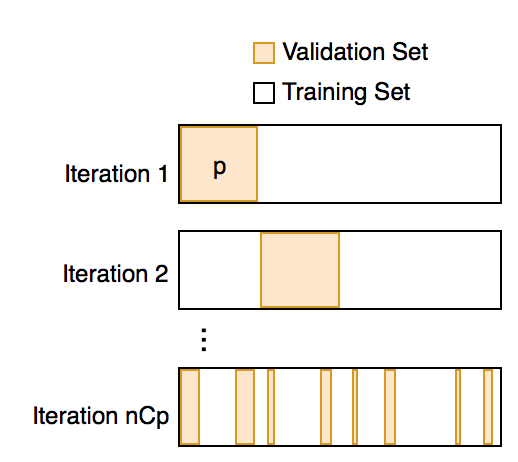
\includegraphics[width=\linewidth]{cross_validation/leavep.png}
	\caption{Leave-p-Out Exhaustive Cross Validation}
\end{marginfigure}
\begin{marginfigure}%
	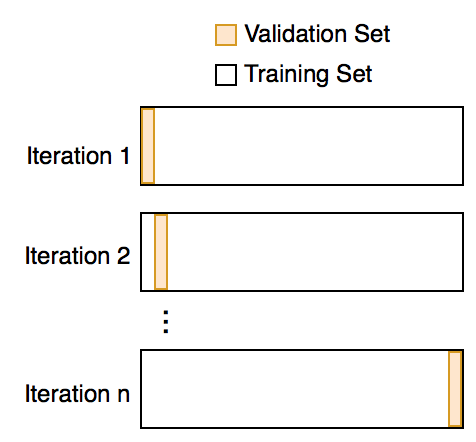
\includegraphics[width=\linewidth]{cross_validation/leave1.png}
	\caption{Leave-One-Out Exhaustive Cross Validation}
	\label{fig:leavep}
\end{marginfigure}

\section{Non-exhaustive cross-validation}

\subsection{Holdout method} \index{cross-validation!holdout}
This method randomly splits the original data set into two sets being the training set and the test set. Usually, the test set is smaller than the training set so that the algorithm has more data to train on. This method involves a single run and so must be used carefully to avoid misleading results. It is therefore sometimes not considered a CV method \citep{kohavi1995study}.

\subsection{$k$-fold} \index{cross-validation!k-fold}
This method randomly splits the original data set into $k$ equally sized subsets, as shown in Fig.~\ref{fig:kfold}. The function is then trained and validated $k$ times, each time taking a different subset as the test data and the remaining $(k-1)$ subsets as the training data, using each of the $k$ subsets as the test set once. The $k$ results are averaged to produce a single estimation. Stratified $k$-fold cross validation is a refinement of the $k$-fold method, which splits the original samples into equally sized and distributed subsets, having the same proportions of the different target labels \citep{kohavi1995study}.

\begin{figure}
  \centering
  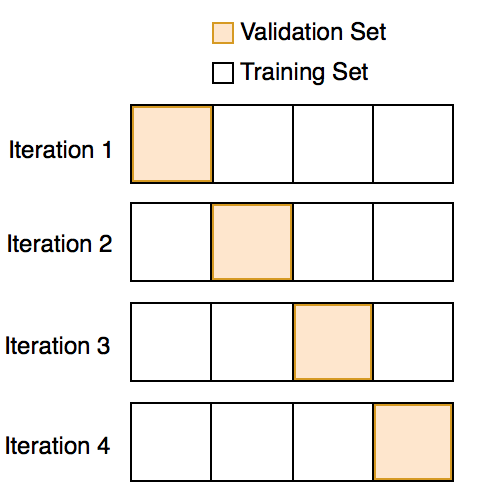
\includegraphics[width=0.5\linewidth]{cross_validation/kfold.png}
  \caption{$k$-Fold Cross Validation where $k$=4}
  \label{fig:kfold}
\end{figure}

\subsection{Repeated random sub-sampling} \index{repeated random sub-sampling}
This method is also known as the Monte Carlo CV. It splits the data set randomly with replacement into training and test subsets using some predefined split percentage, for every run. Therefore, this generates new training and test data for each run but the test data of the different runs might contain repeated samples, unlike that of $k$-fold \citep{xu2001monte}.


All of the above cross-validation methods are used to check whether the model has been overfitted or underfitted and hence estimating the model's ability of fitting to independent data . Such ability is measured using quantitative metrics appropriate for the model and data \citep{kohavi1995study, arlot2010survey}. In the case of classification problems, the misclassification error rate is usually used whilst for regression problems, the mean squared error (MSE) is usually used. MSE is represented by Eq.~\ref{mse}, where n is the total number of test samples, $Y_i$ is the true value of the $i^{th}$ instance and $\hat{Y}_i$ is the predicted value of the $i^{th}$ instance.

\begin{equation}\label{mse}
MSE = \frac{1}{n}\sum^{n}_{i=1}(Y_i - \hat{Y}_i)^2
\end{equation}

Underfitting \index{underfitting} is when the model has a low degree (e.g. $y = x$, where the degree is 1) and so is not flexible enough to fit the data making the model have a low variance and high bias \citep{baumann2003cross}, as seen in Fig.~\ref{fig:models}a. Variance is the model's dependence on the training data and bias is model's assumption about the shape of the data \citep{arlot2010survey}. On the other hand, as seen in Fig.~\ref{fig:models}b, overfitting \index{overfitting} is when the model has a too high degree (e.g. $y = x^{30}$, where the degree is 30) causing it to exactly fit the data as well as the noise and so lacks the ability to generalize \citep{baumann2003cross}, making the model have a high variance. Cross-validation helps reduce this bias and variance since it uses most of the data for both fitting and testing and so helps the model learn the actual relationship within the data. This makes cross-validation a good technique for models to acquire a good bias-variance tradeoff \citep{arlot2010survey}.


\begin{marginfigure}%
	\centering
	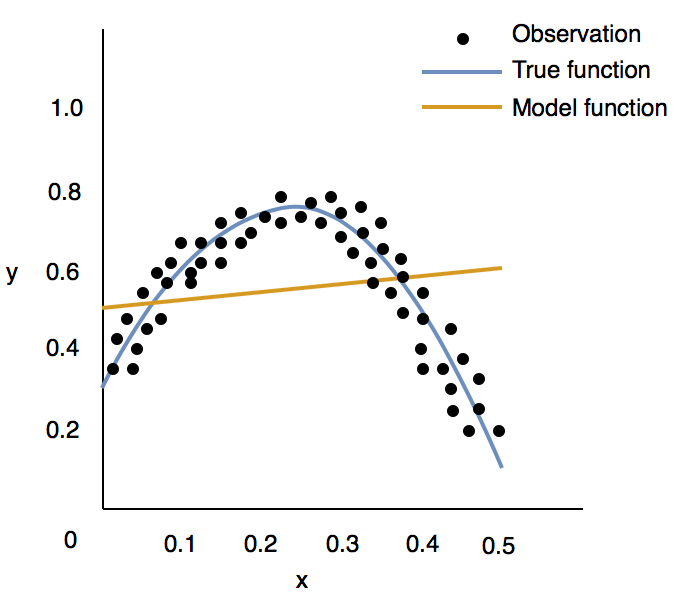
\includegraphics[width=\linewidth]{cross_validation/underfitting.png}
	\caption{Model Underfitting}
\end{marginfigure}
\begin{marginfigure}%
	\centering	
	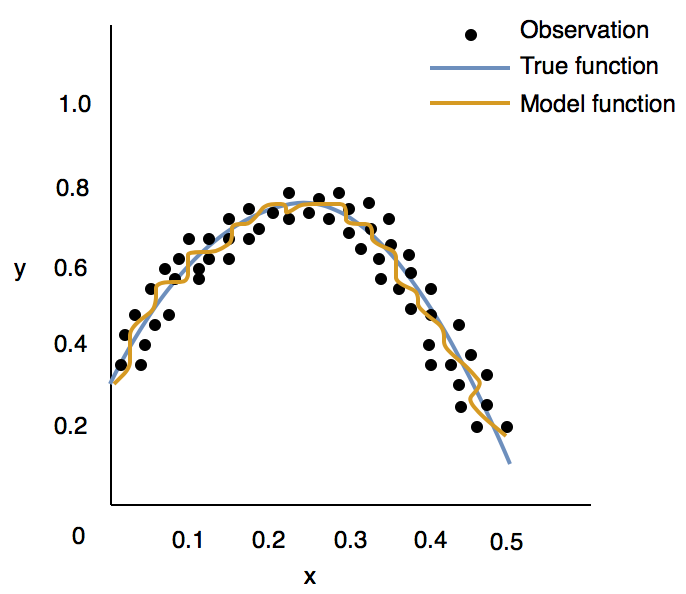
\includegraphics[width=\linewidth]{cross_validation/overfitting.png}
	\caption{Model Overfitting}
	\label{fig:models}
\end{marginfigure}

As stated in \citep{kohavi1995study}, the LOO method gives a 0\% accuracy on the test set when the number of target labels are equal to the number of instances in the dataset. It is shown that the $k$-fold CV method gives much better results, due to its lower variance, especially when $k = {10, 20}$. Furthermore, R. Kohavi et al. state that the best accuracy is achieved when using the stratified cross-validation method, since this has the least bias.

Therefore, lets take an example using the stratified $k$-fold cross-validation method with $k=10$. Let's say that we are trying to solve age group classification, using eight non-overlapping age groups being 0-5, 6-10, 11-20, 21-30, 31-40, 41-50, 51-60, and 61+. We are using the FG-NET labelled data set, which contains around 1000 images of individuals aged between 0 and 69. Before we can start training our model (e.g. CNN), we must divide our data set into training and test subsets and this is where cross validation comes in. Therefore, we start by taking the 1000 images of our data set and splitting them according to their target class. Let us assume we have an equal amount of 125 $(1000/8)$ images per class\footnote{Down-sampling or up-sampling are common techniques used when there is an unequal amount of samples for the different classes.}. As depicted in Fig.~\ref{fig:example}, we can now start forming our 10 folds by taking 10\% of each age-group bucket, randomly without replacement. Hence, we will end up with 10 subsets of 100 images that are equally distributed along all age-groups. With these subsets, we can estimate our model's accuracy with a lower bias-variance tradeoff. Since we are using 10-fold CV, we will train and test our model 10 times. For the first iteration, we shall use subset 1 as the validation set and subsets 2 to 10 as the training set, for the second iteration we use subset 2 as the test set and subsets 1 plus 3 to 10 as our training set, and so on (as shown in Fig.~\ref{fig:kfold}). For each iteration we use the misclassification error rate to obtain an accuracy value and we finally average the 10 accuracy rates to obtain the global accuracy of our model when solving age group classification, given the FG-NET data set. Hence, we have now estimated the prediction error of the model and have an idea of how well our model performs in solving such a problem. It is important to note that cross-validation is \textit{just} an estimation method and when using our model in real-life applications we do not apply CV but rather train our model with all the data we have.

\begin{figure*}
\centering
  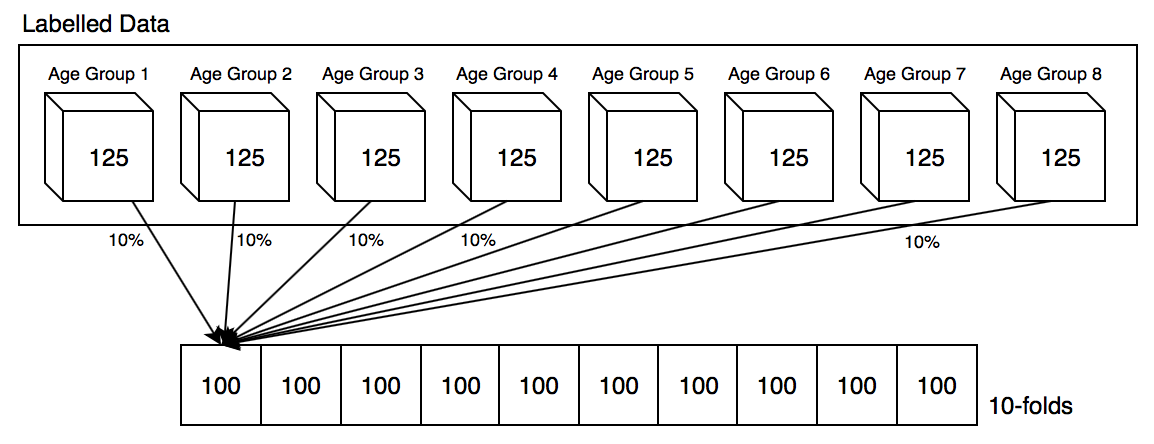
\includegraphics[width=0.88\linewidth]{cross_validation/example-cv.png}
  \caption{Stratified 10-fold cross-validation on 1000 labelled images of 8 different classes}
  \label{fig:example}
\end{figure*}

As concluded by \citet{varma2006bias}, cross-validation is well implemented when everything is taken place within every CV iteration (including preprocessing, feature-selection, learning new algorithm parameter values, etc.), and the least bias can be achieved when using nested CV methods.

\index{cross-validation|)}